\documentclass[a4paper,11pt]{article}
%@@@@@@@@@@@@@@@@@@@@@@@@@@@@@@@@@@@@@@@@@@@@@@@@@@@@@@@@@@@
%@@@@@@@@@@@@@@@@      PACOTES BÁSICOS		     @@@@@@@@@@
%@@@@@@@@@@@@@@@@@@@@@@@@@@@@@@@@@@@@@@@@@@@@@@@@@@@@@@@@@@@

\usepackage[T1]{fontenc}
\usepackage[utf8]{inputenc}
\usepackage{lmodern} 
\usepackage[portuguese]{babel}
\usepackage{amsmath}
\usepackage{array}
\usepackage{graphicx}				%para imagens
\usepackage{epstopdf} 				%resolve problemas eps-pdf
\usepackage{pict2e}				%%writting to images
%@@@@@@@@@@@@@@@@@@@@@@@@@@@@@@@@@@@@@@@@@@@@@@@@@@@@@@@@@@@
%@@@@@@@@@@@@@@@@     PACOTES NÃO TAOBÁSICOS		 @@@@@@@@@@
%@@@@@@@@@@@@@@@@@@@@@@@@@@@@@@@@@@@@@@@@@@@@@@@@@@@@@@@@@@@
\usepackage{fancyhdr}				% para o cabeçalho bonito
\usepackage{caption}					%para legendas
\usepackage{subcaption}				% e sublegendas
\usepackage{placeins} 				%controlar o lugar dos floats
\pagestyle{fancy} 					% número de pag e cabeçalho
\usepackage{txfonts} 				%fontes bonitas? acho que para o título
\usepackage[usenames]{color} 		% algo com gunplot e eps
\usepackage{ifthen}
\usepackage{xparse}
\graphicspath{{./../images/}{./../data/}{./graph/}}	% procura imagens nessa pasta
\usepackage{float} %%para definir ambiente gráfico
\newfloat{Gráfico}{hbtp}{lop}[section]
%\usepackage{undertilde}	%%para notação de vetor do yuri
\usepackage[import]{xy} % para escrever em imagens
\xyoption{import}

\usepackage{listings}
\lstset{frame=single,}
%@@@@@@@@@@@@@@@@@@@@@@@@@@@@@@@@@@@@@@@@@@@@@@@@@@@@@@@@@@@
%@@@@@@@@@@@@@@@@      Cabeçalho de cada página      @@@@@@@
%@@@@@@@@@@@@@@@@@@@@@@@@@@@@@@@@@@@@@@@@@@@@@@@@@@@@@@@@@@@
\setlength{\headheight}{25pt}%compila sem erro
	\fancyhead{}
	\fancyfoot{}
	\fancyhead[R]{Sistemas de Medição}%direito superior
	\fancyhead[L]{
\includegraphics[height=0.25in]{./../images/logo_unb.pdf}}%esquerda superior
	\fancyfoot[C]{\thepage}%baixo centro
%E: Even page, O: Odd page, L: Left field, C: Center field, R: Right field, H: Header, F: Footer
% em documentos com dois lados use LO, RO. como esse documento não tem lados essa opção é inútil


%@@@@@@@@@@@@@@@@@@@@@@@@@@@@@@@@@@@@@@@@@@@@@@@@@@@@@@@@@@@
%@@@@@@@@@@@@@@@@      NOVOS COMANDOS		      @@@@@@@@@
%@@@@@@@@@@@@@@@@@@@@@@@@@@@@@@@@@@@@@@@@@@@@@@@@@@@@@@@@@@@
\newcommand\undermat[2]
	{
	  \makebox[0pt][l]
	  	{$\smash{\underbrace{\phantom{%
    \begin{matrix}#2\end{matrix}}}_{\text{$#1$}}}$
    		}#2
    	}
    	
\newcommand{\HRule}
	{
	\rule{\linewidth}{0.5mm}
	}
	
\newcommand{\EmptyPage}
	{
	\thispagestyle{empty}
	\mbox{ }
	\newpage	
	} 
	
\newcommand{\MakeMyTitlePage}[4]
%%Argumentos: 
%1º Nome da Matéria
%2º subtítulo ex: experimento IV
%3º título
%4º autores
% exemplo de autores:
%	\begin{center} \large
%		\begin{tabular}{llr} \
%		& & \\[0.05cm]		
%		Professora & Nadia Maria de Liz Koche & \\
%		
%		Alunos:& & \\
%		& Juarez A.S.F 					& 11/0032829\\
%		& Sérgio Fernandes da Silva Reis & 11/0140257\\
%		& Jedhai Pimentel				& 09/0007883\\	[0.05cm]	
%		\end{tabular}
%	\end{center}
{
\begin{titlepage}
\begin{center}

% Upper part of the page. The '~' is needed because \\
% only works if a paragraph has started.

\includegraphics[width=\textwidth]{./../images/logo_unb.pdf}~\\[1cm]

\Huge #1\\[0.5cm]

\huge #2

% Title
\HRule \\[0.4cm]
{ \huge \bfseries  #3}\\[0.4cm]

\HRule \\[0.5cm]

{\large \today}


\vfill %%o que vier depois vai ao fim da páginda


%Autor e Professor
\begin{center} \large
#4
\end{center}

\end{center}
\end{titlepage}

\EmptyPage
\tableofcontents
\newpage

}
	
%@@@@@@@@@@@@@@@@@@@@@@@@@@@@@@@@@@@@@@@@@@@@@@@@@@@@@@@@@@@
%@@@@@@@@@@@@@@@@      NOVOS AMBIENTES		      @@@@@@@@@
%@@@@@@@@@@@@@@@@@@@@@@@@@@@@@@@@@@@@@@@@@@@@@@@@@@@@@@@@@@@
\newcounter{graph-c}
\setcounter{graph-c}{0}


%\NewDocumentEnvironment{Graph}{m}
 % {%antes
  %\addtocounter{graph-c}{1}
  %\begin{figure}
  %}
 %{
 %depois
%	\end{figure} 
%	\caption*{Grafico \arabic{graph-c} - #1}
 %}

















%inclui todosos pacotes utilizados

\newcommand{\MyBox}[1]
{
	\begin{tabular}{|l|}\hline
	  #1 \\ \hline	    
	\end{tabular} 	
}

\lstset{frame=single,}	

\begin{document}



\MakeMyTitlePage
{Análise Dinâmica Linear}
{Experimento III}
{Plantas Servo de Movimento Linear e Rotacional}
{%autores
		\begin{tabular}{llr} \
		& & \\[0.05cm]		
		Professor & Henrique Cezar Ferreira & \\
		
		Alunos:& & \\
		& Juarez A.S.F 												& 11/0032829\\
		& Luís Henrique Vieira Amaral						&	10/0130488 	
			\end{tabular}
}

%@@@@@@@@@@@@@@@@@@@@@@@@@@@@@@@@@@@@@@@@@@@
%@@@@@@@@@@@@@@@@      OBJETIVOS      @@@@@@@@@@@@@@@@@@
%@@@@@@@@@@@@@@@@@@@@@@@@@@@@@@@@@@@@@@@@@@@
\section{Objetivos}
\paragraph{} O experimento visa a familiarização com as plantas servo de movimento linear e rotacional da
Quanser, o reconhecimento de suas principais peças e a utilização de sua interface com o simulink do matlab.
%@@@@@@@@@@@@@@@@@@@@@@@@@@@@@@@@@@@@@@@@@@@@@
%@@@@@@@@@@@@@@        INTRODUÇÃO       @@@@@@@@@@@@@@@@@@@@ 
%@@@@@@@@@@@@@@@@@@@@@@@@@@@@@@@@@@@@@@@@@@@@@
\section{Introdução Teórica}
\paragraph{}No processo de controle de sistemas físicos estamos interessados em monitorar certas quantidades
e decidirmos sobre ações a serem aplicadas sobre o sistema de forma a controlar seu funcionamento.Em muitos
sistemas de controle comparamos o estado atual com o estado desejado e então atuamos sobre o sistema de modo
a empurrar o estado do sistema na direção  daquele desejado. É de muito interesse que esse processo
 seja feito de forma automática e
para isso o uso de computadores se torna recorrente. 
    
\paragraph{} Neste experimento, entramos em contato com uma plantas servo de movimento linear e rotacional com interface de controle e monitoramento via conexão usb. A planta em questão faz parte de um kit da empresa Quanser especialmente
projetado para o uso em estudo de sistemas de controle. O conjunto consiste em uma placa de aquisição de dados,
um módulo de potência, a planta propriamente e um pacote de softwares integrados com o matlab para permitir
fácil conexão e manipulação através do computador. Trabalhamos com duas plantas em particular: uma para 
movimento linear e outra para movimento angular. A partir do software de controle QUARC-Simulink pode-se 
simular, monitorar e controlar o estado da planta
  
\paragraph{}Para o controle da planta faz-se necessário o uso do módulo de potência e conversores 
Digital para Analógico (DA) e Analógico para Digitar (AD). Para o monitoramento
utiliza-se os encoders presentes na planta e sua calibração por meio dos corretos parâmetros de ganho.
As principais peças do kit são mostradas nas figuras \ref{fig:aquisicao}, \ref{fig:pot_mod}, \ref{fig:planta_rot}
e \ref{fig:planta_lin}.

\paragraph{} A utilização do computador traz benefícios no sentido de fornecer maior precisão e melhoria na interface com o
 usuário, além de permitir gerenciar e supervisionar processos à distância.
\FloatBarrier
\begin{figure}[!htp]
\centering
	\begin{tabular}{ll}
		\begin{subfigure}[!htp]{0.3\textwidth}
			\centering
			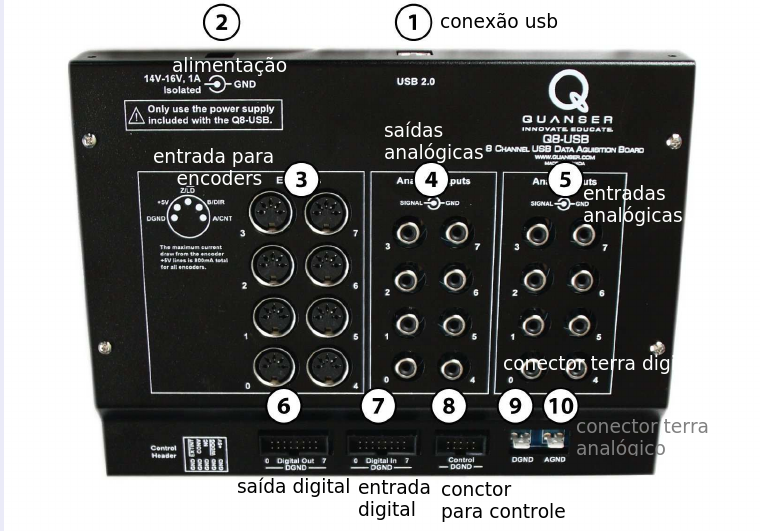
\includegraphics[scale = 0.2]{./../images/dataAquisitoinBoard.png}
			\caption{placa de aquisição de dados}
			\label{fig:aquisicao}
		\end{subfigure}		&
		\begin{subfigure}[!htp]{0.3\textwidth}
			\centering
			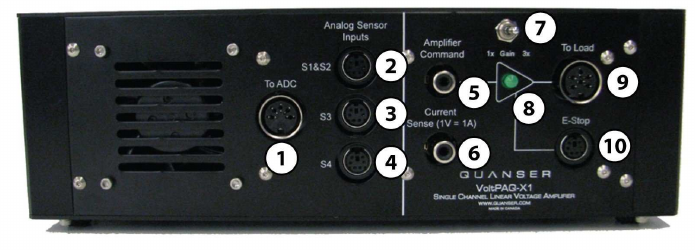
\includegraphics[scale = 0.2]{./../images/EnergyBoard.png}
			\caption{módulo de potência}
			\label{fig:pot_mod}
		\end{subfigure}		\\
		\begin{subfigure}[!htp]{0.3\textwidth}
			\centering
			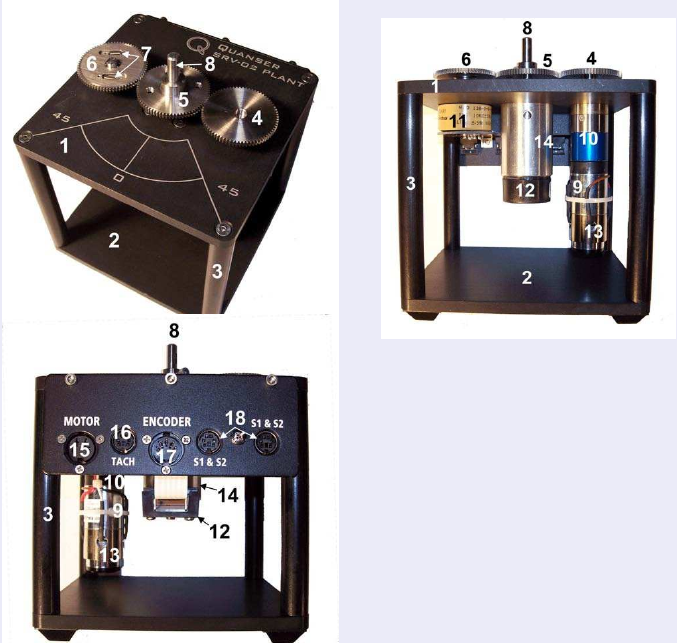
\includegraphics[scale = 0.2]{./../images/plantaRotatoria.png}
			\caption{planta rotatória}
			\label{fig:planta_rot}
		\end{subfigure}		&
		\begin{subfigure}[!htp]{0.3\textwidth}
			\centering
			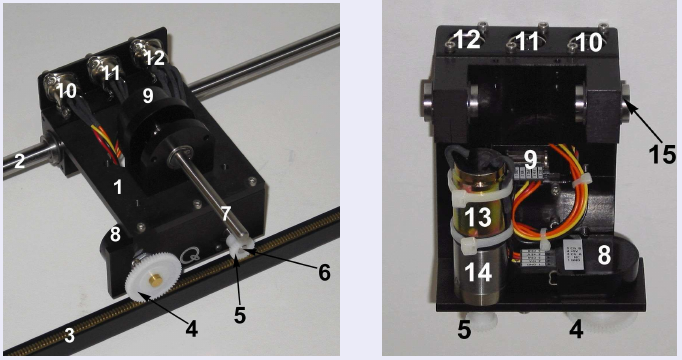
\includegraphics[scale = 0.2]{./../images/plantaLinear.png}
			\caption{planta linear}
			\label{fig:planta_lin}
		\end{subfigure}		\\
	\end{tabular}	
\caption{Principais módulos do kit}
\end{figure}
\FloatBarrier

%@@@@@@@@@@@@@@@@@@@@@@@@@@@@@@@@@@@@@@@@@@@
%@@@@@@@@@@@@       PROCEDIMENTOS        @@@@@@@@@@@@@@@@@@
%@@@@@@@@@@@@@@@@@@@@@@@@@@@@@@@@@@@@@@@@@@@
\newpage
\section{Descrição Experimental}
\begin{itemize}
\item Inicialmente montamos o esquemático no simulink como na figura\ref{fig:montagem1}. Compilamos
o código e iniciamos o comando. Nessa primeira etapa desejamos apenas observar um movimento 
senoidal na planta para nos familiarizarmos com os procedimentos.

\item Estando familiarizado com o funcionamento da planta montamos o diagrama como na figura
\ref{fig:montagem2}. Os ganhos devem ser corretamente ajustados para cada sensor. São eles:
	\begin{itemize}
		\item para o \textbf{potenciômetro} : 35.2 graus/V
		\item para o \textbf{tacômetro}(utilizamos a engrenagem maior) : 9.5238 RPN/V
		\item para o \textbf{encoder }: 0.087891 graus/V
	\end{itemize}
\end{itemize}
Antes de compilar setamos o bloco osciloscópio para salvar os dados na área de trabalho no formato
array. Com o programa compilado e rodando movemos manualmente o pinhão maior da planta e 
observamos a resposta no simulink. Encerramos a simulação e, com os dados salvos na área de 
trabalho, plotamos o resultado obtido.
\FloatBarrier
\begin{figure}[!htp]
\centering
	\begin{tabular}{l}
		\begin{subfigure}[!htp]{0.5\textwidth}
			\centering
			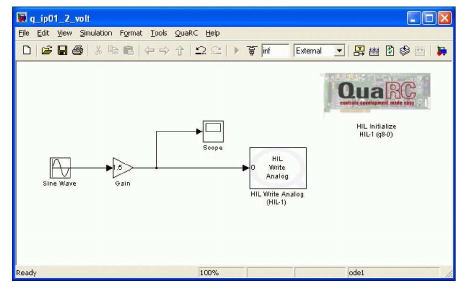
\includegraphics[scale = 0.7]{./../images/montagem1.png}
			\caption{montagem inicial}
			\label{fig:montagem1}
		\end{subfigure}		\\
		\begin{subfigure}[!htp]{0.5\textwidth}
			\centering
			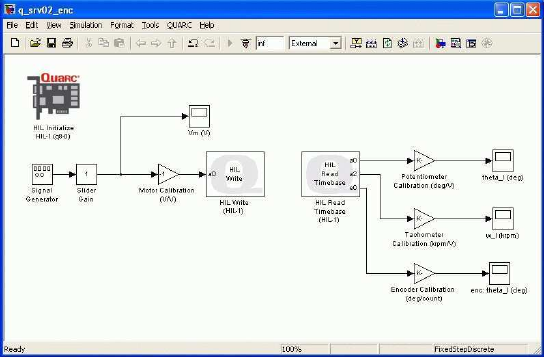
\includegraphics[scale = 0.7]{./../images/montagem2.png}
			\caption{segunda montagem}
			\label{fig:montagem2}
		\end{subfigure}
	\end{tabular}
\caption{blocos esquemáticos para o simulink}
\end{figure}
\FloatBarrier

%@@@@@@@@@@@@@@@@@@@@@@@@@@@@@@@@@@@@@@@@@@@@@@@@
%@@@@@@@@@@@@@@@@@@@       DADOS      @@@@@@@@@@@@@@@@@@@@@@
%@@@@@@@@@@@@@@@@@@@@@@@@@@@@@@@@@@@@@@@@@@@@@@@@
 \section{Resultados}
\paragraph{} Os resultados obtidos na segunda etapa do procedimento são mostrados nos gráficos a seguir.

\FloatBarrier
\begin{figure}[!htp]
\begin{tabular}{ll}
	\begin{subfigure}[!htp]{0.5\textwidth}
		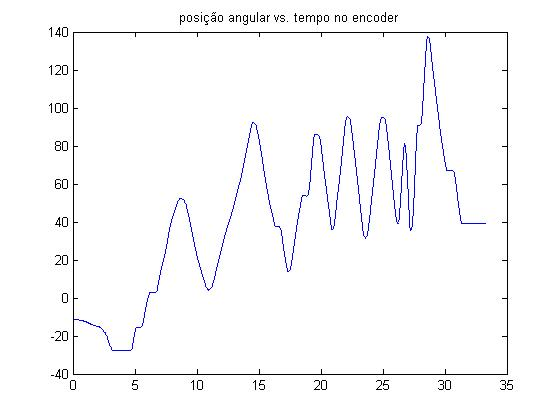
\includegraphics[scale=0.4]{./../images/theta_enc.jpg}
		\caption{posição angular no encoder}
		\label{fig:output-angular-encoder}
	\end{subfigure}
	&
	\begin{subfigure}[!htp]{0.5\textwidth}
		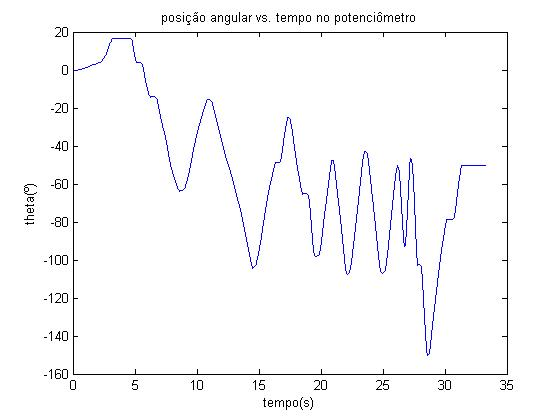
\includegraphics[scale=0.4]	{./../images/theta_pot.jpg}
		\caption{posição angular no potenciômetro}
		\label{fig:output-angular-pot}
	\end{subfigure} 
	\\
	\begin{subfigure}[!htp]{0.5\textwidth}
		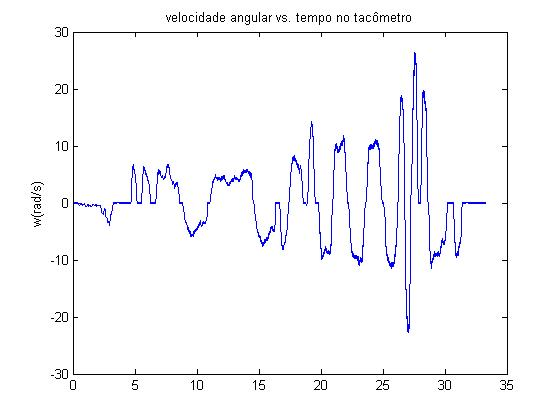
\includegraphics[scale=0.4]	{./../images/w_tac.jpg}
		\caption{velocidade angular no tacômetro}
		\label{fig:output-vel-ang-tac}
	\end{subfigure}
\end{tabular}		
\end{figure}
\FloatBarrier

%@@@@@@@@@@@@@@@@@@@@@@@@@@@@@@@@@@@@@@@@@@@
%@@@@@@@@@@@@@@       Análise         @@@@@@@@@@@@@@@@@@@@@@
%@@@@@@@@@@@@@@@@@@@@@@@@@@@@@@@@@@@@@@@@@@@@
\newpage
\section{Discussão}
\paragraph{} Notamos nos gráficos obtidos uma inversão de polaridade entre os sinais obtidos 
do encoder e do potenciômetro. Para corrigir isso podemos multiplicar por -1 o ganho de um
dos dois sensores.

\paragraph{}Respondemos a seguir as perguntas deixadas como exercício para o relatório.

\subsection{Questão 1}
	\paragraph{} O acionamento das plantas IP02(linear) ou SRV02(rotacional) é feito apartir do módulo 
	de potência VoltPAQ e esta
	é acionada pela placa de aquisição de dados Q8-USB. O computador por sua vez está ligado via USB na 
	placa de aquisição e deve também jogar o sinal de controle no canal D/A desta.
	
\subsection{Questão 2} 
	\paragraph{}A planta linear possui 2 sensores e a angular 3; ambas possuem apenas um atuador.Nominalmente temos:
	\begin{itemize}
		\item planta linear(IP02)
			\begin{itemize}
				\item sensores:
					\begin{enumerate}
					\item encoder de posição linear do carro
					\item encoder de posição do pêndulo
					\end{enumerate}
				\item atuador:
					\begin{enumerate}
						\item motor CC
					\end{enumerate}
			\end{itemize}

		\item planta angular(SRV02)
			\begin{itemize}
				\item sensores:
					\begin{enumerate}
					\item encoder de posição angular
					\item potenciômetro de posição angular
					\item tacômetro para velocidade angular
					\end{enumerate}
				\item atuador:
					\begin{enumerate}
						\item motor CC
					\end{enumerate}
			\end{itemize}

			
	\end{itemize}
\subsection{Questão 3}
\paragraph{} A conversão do movimento rotacional em movimento retilíneo é feito a partir do conjunto motor, pinhão, eixo e cremalheira. O movimento rotacional do motor é transmitido para o eixo e este o passa para o pinhão. O atrito entre
o pinhão e a cremalheira na região de contato empurra o carrinho para a frente, transformando o movimento inicialmente
rotacional do conjunto em linear. Supondo que não haja deslizamento entre as partes, a velocidade angular do motor 
$\omega$ é igualmente transmitida para o eixo e para o pinhão e a relação entre a rotação do pinhão de raio $r$ e a 
velocidade linear $v$ da planta é dada por:
\begin{equation}
	v = \omega \cdot r
\end{equation}
\subsection{Questão 4}
\paragraph{} O sinal de ganho nos encoders e nos sensores é de extrema importância pois permite uma correta
leitura e interpretação dos dados. Cada sensor apresenta uma saída indireta que muitas vezes é tensão ou corrente.
Essas tensões ou correntes estão relacionadas com a variável sendo medida e as características internas 
do sensor. É justamente o sinal de ganho que faz a conexão entre esses dois mundos: a variável sendo medida
e a resposta em tensão ou corrente do sensor. Por exemplo, tome um potenciômetro utilizado para medição de 
deslocamento angular. Ao ligarmos um ohmímetro em seus terminais estamos de fato medindo resistência, mas 
se conhecermos como sua resistência varia em função do ângulo, por exemplo, segundo a relação 
$R(\theta) = R_0 + \alpha \theta $, podemos inverter a relação para obter $\theta$.

\subsection{Questão 5}

\begin{itemize}
	\item 
O bloco \textbf{HIL Initialize} tem o propósito de configurar o dispositivo de aquisição de dados
	\item 
O bloco\textbf{ HIL Write Analog} tem a função de fornecer um sinal de tensão na saída do conversor digital/analógico da placa de aquisição de dados.
	\item 
O bloco \textbf{HIL Read Encoder Timebase} pode ser ajustado para ler o canal da placa de aquisição de dados referente à entrada do encoder, potenciômetro e tacômetro.
\end{itemize}
\subsection{Questão 6}
\paragraph{}Para limitar a tensão máxima que atua sobre o motor CC podemos utilizar um bloco de \textbf{MinMax}
imediatamente antes do bloco \textbf{ HIL Write Analog}. Esse bloco possui permite escolher a funcionalidade
de mínimo ou máximo entre sinais e o número de entradas. Para limitarmos superiormente o sinal selecionamos
o modo de mínimo e 2 canais de entrada. Em um dos canais jogamos um sinal constante e igual a valor máximo 
desejado, no outro jogamos o sinal que queremos filtrar. Dessa forma, se o sinal entrado for menor que 
o mínimo ele passa pelo filtro, se for maior ele é retido e apenas o valor limitante desejado é passado para o
motor. De forma análogo poderíamos projetar um filtro de tensão mínima utilizando a funcionalidade de máximo
desse bloco. Ligando esses dois filtros em série obtemos um filtro de banda, onde temos certeza de que o sinal
estará entre dois valores estabelecidos.
%@@@@@@@@@@@@@@@@@@@@@@@@@@@@@@@@@@@@@@@@@@@@@
%@@@@@@@@@@@@@@       Conclusão         @@@@@@@@@@@@@@@@@@@@@@
%@@@@@@@@@@@@@@@@@@@@@@@@@@@@@@@@@@@@@@@@@@@@@

\newpage
\section{Conclusão}

\paragraph{} O experimento permitiu utilizar os kits de movimento linear e rotacional da Quanser,
conhecer suas principais peças, funcionalidades e utilizar sua interface com o matlab. Por meio da interface
com o matlab e da correta calibração de ganho dos encoders e sensores
foi possível obter gráficos para as posições e velocidades angulares da planta rotacional.
Ao final, utilizou-se as ferramentas do simulink para projetar um sinal de controle limitado a valores máximos
e mínimos previamente definidos.

%@@@@@@@@@@@@@@@@@@@@@@@@@@@@@@@@@@@@@@@@@@@@@@
%@@@@@@@@@@@@@@       REFERÊNCIAS     @@@@@@@@@@@@@@@@@@@@@@
%@@@@@@@@@@@@@@@@@@@@@@@@@@@@@@@@@@@@@@@@@@@@@@
\begin{thebibliography}{9}    
	 \bibitem{ADL-NISE}
  		Nise, N.S.
  		\emph{Engenharia de Sistemas de Controle}
 		 5ª ed.
		LTC, 2009.

	 \bibitem{ADL-OGATA}
  		Ogata, K.
  		\emph{Moder Control Engeeniring}
 		 5ª ed.
		Pearson, 2010.
	 
\end{thebibliography}
\end{document}
